\documentclass{article}

\usepackage[T1]{fontenc}
\usepackage[utf8]{inputenc}
\usepackage[polish]{babel}
\usepackage[a4paper]{geometry}
\usepackage{enumerate}
\usepackage[rounded]{syntax}
\usepackage{listings}
\usepackage{graphicx}

\setlength{\grammarparsep}{0pt}

\title{TKOM\\
	Język do operacji na listach}
\author{Marcin Puc}
\date{}

\begin{document}

\maketitle

\section{Opis}
	Celem tego projektu jest stworzenie języka pozwalającego na operowanie na listach. Listy to \textit{sekwencje} obiektów pewnego typu, tj. kolekcje utrzymujące swoje elementy w pewnej kolejności.
	Opracowywany język ma za zadanie umożliwiać operacje takie jak łączenie list, dostęp do elementów listy, wykonywanie potokowych operacji na elementach listy itp.

\section{Funkcjonalności}
	\begin{enumerate}[a)]
		\item wbudowany interpreter
		\item typy danych:
			\begin{itemize}
				\item{\textbf{List}}

					Sekwencja obiektów (możliwie więcej niż jednego typu)
				\item{\textbf{Int}}

					Typ całkowitoliczbowy ze znakiem
				\item{\textbf{Bool}}

					Typ przechowujący wartości logiczne
					\textit{True} i \textit{False}
				\item{\textbf{Func}}

					Obiekt funkcyjny, przechowujący sekwencję operacji
					z możliwymi parametrami;
					opcjonalnie zwraca wartość o jednym z powyższych typów
			\end{itemize}
		\item silna, dynamiczna typizacja danych

			Typ obiektu nie może ulec niespodziewanej konwersji,
			lecz pojęcie typu pojawia się dopiero na poziomie
			uruchomienia programu;
			podobnie jak w języku Python identyfikatory na poziomie kodu źródłowego
			stanowią \textit{etykiety} które mogą być przepinane między
			rzeczywistymi obiektami
	\end{enumerate}
	
\begin{figure}
	\centering
		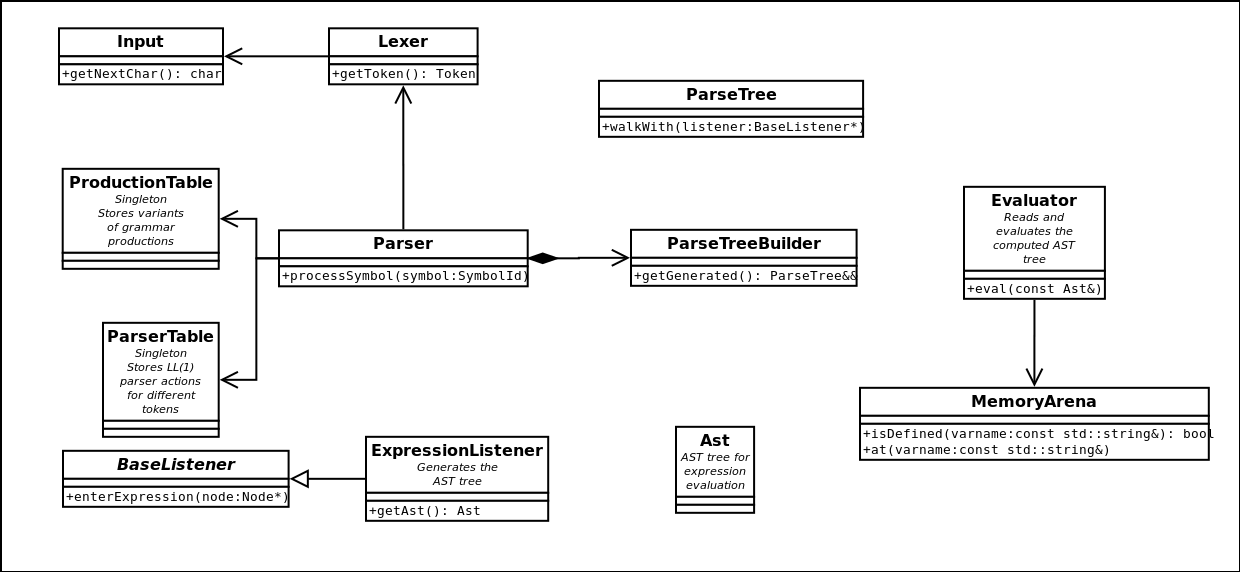
\includegraphics[scale=0.4]{diagrams/architecture.png}
	\caption{Główna architektura programu}
\end{figure}

\break
\section{Specyfikacja techniczna}

\subsection{Środowisko programistyczne}
	Projekt będzie wykonany w języku C++. Mogą zostać wykorzystane zewnętrzne biblioteki, np. \textit{Catch2} (testy jednostkowe), \textit{cxxopts} (argumenty wiersza poleceń).

\subsection{Interpreter}
	Obsługa języka należy do programu REPL (Read Evaluate Print Loop) --- język jest interaktywnie interpretowany. Program ten działa w trybie tekstowym.

	REPL wyświetla znak zachęty, wczytuje ze standardowego wejścia polecenie, interpretuje je i wyświetla jego wynik. W przypadku gdy polecenie zajmuje więcej niż jedną linię, interpreter sygnalizuje ten fakt zmianą znaku zachęty.

	W przypadku wystąpienia błędu na etapie analizy składniowej lub interpretacji, REPL wyświetla odpowiedni komunikat o błędzie.
\subsection{Operacje `potokowe'}

	Język obsługuje dwie kluczowe operacje na listach: \textit{map} i \textit{filter}, zapisywane operatorami odpowiednio `\verb|>:|' i `\verb|>?|'.
	Operacje te przyjmują jako argument jednoargumentowe obiekty funkcyjne (dla \textit{filter} obiekt ten musi zwracać typ Bool).

\textit{Map} podaje kolejne elementy listy do obiektu funkcyjnego
i zwraca nową listę ze zmodyfikowanymi elementami.

\textit{Filter} podaje kolejne elementy listy do obiektu funkcyjnego
i dodaje je do nowej listy jeżeli obiekt funkcyjny zwróci wartość True.

\subsection{Sposób uruchomienia}

Program działa w trybie interaktywnego REPLa. Aby zbudować projekt należy mieć zainstalowany program \emph{SCons}. Następnie uruchamiamy polecenie \texttt{scons}. Buduje ono projekt i umieszcza plik wykonywalny \texttt{langust} w katalogu \texttt{bin/release/}. Uruchamiamy program i możemy wpisywać polecenia. Aby zakończyć program, należy przesłać sygnał EOF (Ctrl+D na systemie *nix).

\section{Przykłady}
W poniższych przykładach linijki `\verb|$ ...|' i `\verb|> ...|'
oznaczają kod wprowadzany przez użytkownika, a pozostałe
--- odpowiedzi interpretera.

\begin{lstlisting}[frame=tb, title={Operacje na typach prostych}]
$ 2 + 2;
4
$ 5 / 2;
2
$ 100 * 2 - 1;
199
$ 2 + 2 > 5;
False
$ 2 + 2 > 5 || True;
True
\end{lstlisting}
\begin{lstlisting}[frame=tb, title={Pobieranie elementów listy}]
$ l = [0, 1, 2, 3];
[ 0, 1, 2, 3 ]
$ l[1];
[ 1 ]
$ l[1:2];
[ 1, 2 ]
$ l[1:];
[ 1, 2, 3 ]
$ l[:2];
[ 0, 1, 2 ]
\end{lstlisting}
\begin{lstlisting}[frame=tb, title={Operacje \textit{map} i \textit{filter}}]
$ l = [0, 1, 2, 3];
[ 0, 1, 2, 3 ]
$ l >: func(el) {return el+1;};
[ 1, 2, 3, 4 ]
$ l >? func(el) {return el < 2;};
[ 0, 1 ]
\end{lstlisting}
\break
\begin{lstlisting}[frame=tb, title={Obiekty funkcyjne}]
$ f = func(list) {
>  return list >: func(l) {
>                           return l >? func(el) {return el > 2;}
>                                    >: func(el) {return el + 1;};
>                         };
> };
$ l = [[1, 2], [3, 4]];
[ [ 1, 2 ], [ 3, 4 ] ]
$ f.(l);
[ [ ], [ 4, 5 ] ]
\end{lstlisting}

\section{Gramatyka}
	Poniżej znajduje się opis gramatyki w notacji EBNF. Symbolem startowym jest \textit{statement}.

	\renewcommand{\syntleft}{\normalfont\itshape}
	\renewcommand{\syntright}{}

	\begin{grammar}
		<statement> = <expr>, `;' ;

		<statement list> = <statement>, \{<statement>\} ;

		<return stmt> = `return', <expr>, `;' ;

		<parameter list> = <identifier>, \{`,', <identifier>\} ;

		<func literal> = `func', `(', [<parameter list>], `)',
						`{', [<statement list>], [<return stmt>], `}' ;
	\end{grammar}
	\begin{grammar}
		<alpha> = ? "A-Z" or "a-z" ? ;

		<non-zero digit> = ? "1-9" ? ;

		<digit> = `0' | <non-zero digit> ;

		<alphanum> = <alpha> | <digit> ;

		<boolean> = `False' | `True' ;

		<natural number> = <non-zero digit>, \{<digit>\} ;

		<integer> = `0' | [`-'], <natural number> ;

		<identifier> = (<alpha> | `_'), \{<alphanum> | `_'\} ;

		<pipe op> = `>?' | `>:' ;

		<mul op> = `*' | `/' | `%' ;

		<add op> = `+' | `-' ;

		<rel op> = `<' | `<=' | `>' | `>=' ;

		<eq op> = `==' | `!=' ;
	\end{grammar}
	\begin{grammar}
		<list literal> = `[', [<arglist>], `]' ;

		<list index> = `:', <expr> | <expr>, [`:', [<expr>]] ;

		<func apply> = <identifier>, `.', `(', [<arglist>] `)' ;

		<arglist> = <expr>, \{`,', <expr>\} ;

		<atom> = <integer> | <boolean> | <list literal>
				 | <func apply> | <func literal> | <identifier> | `(', <expr>, `)' ;
	\end{grammar}
	\begin{grammar}
		<list expr> = <atom>, \{<pipe op>,
					  (<identifier> | <func literal>)
					  | `[', <list index>, `]'\} ;

		<mul expr> = <list expr>, \{<mul op>, <list expr>\} ;

		<add expr> = <mul expr>, \{<add op>, <mul expr>\} ;

		<rel expr> = <add expr>, [<rel op>, <add expr>] ;

		<eq expr> = <rel expr>, [<eq op>, <rel expr>] ;

		<not expr> = [`!'], <eq expr> ;

		<and expr> = <not expr>, \{`&&', <not expr>\} ;

		<or expr> = <and expr>, \{`||', <and expr>\} ;

		<expr> = <or expr>, [`=', <or expr>] ;
	\end{grammar}

\end{document}